\documentclass{article}
\usepackage{graphicx} 
\title{30 Mark question prep(Assumes the practical will be asked)}
\author{MJ Bezuidenhout}
\begin{document}
\maketitle
\section{Database design}
The purpose of this project is to design an online shopping platform with multiple users, stores, cart-checkout, stock management and transaction recording. 
The following Logical entities need to be considered for the database design:
\begin{description}
\item[Users] People who trade in the shopping platform. Associated with login credentials, shops, transactions and carts
\item[Products] Aside from logical attributes like price and color, the products are associated with a store and are refered to by carts
\item[Stores] Associated with users, contains products. 
\item[Carts] Associated with a session, contains products.
\end{description}  
Furthermore, the following tables relate to the management of these logical entities:
\begin{description}
\item[Sessions] A unique identifier that prevents a PHP session from being hijacked, without necessitating user authentication on every page.
\item[Transactions]Associated with users and amounts. 
\end{description}


\section{ERD}
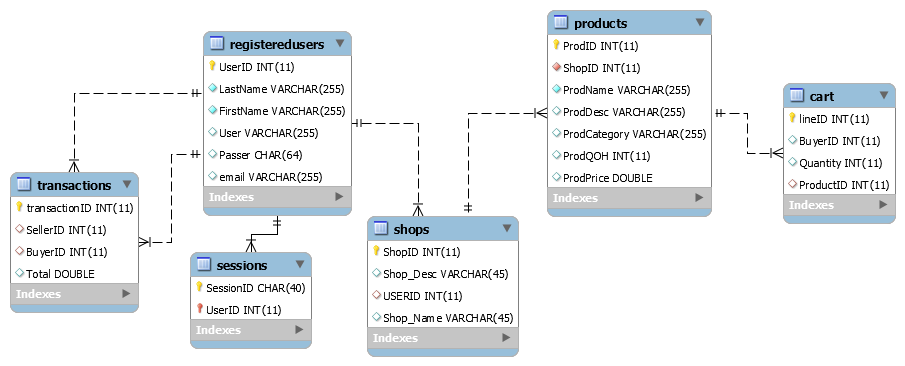
\includegraphics[width=1\textwidth]{ERD}
\section{Web interface}
\subsection{Security(SQL,PHP)}
\begin{description}
	\item[Session management] The session identifier is generated using an encrypted combination of the system time and a random string. This identifier is associated with the authenticated user and this association is confirmed on every page, as part of the header. 
	\item[User Authentication] User passwords are stored encrypted. It is generally understood that this does not have much of an impact on security, but it is a privacy concern if site admins have access to user passwords.
	\item[User Registration] Users register using an HTML form. All fields are set up to prevent sql injection. Furthermore, content checking is done to constrain things like email validity, username availability and password length
	\item[Transaction management(external)] The site will be designed to make use of an external transaction service, like PayFast Secure.
\end{description}

\subsection{User Friendliness(HTML,PHP)}
\begin{description}
	\item[Header] The header used for session management is also used to present the authenticated user with useful links (CSS Styled as buttons) to relevant pages
	\item[Forms] The forms have a familiar feel and fields can by cycled through using the tab key. Where possible, different browsers will be tested for autocomplete behavior
	\item[Readable URL's] Unless security/privacy is a concern, GET will be used in stead of POST in order to keep the browser's ``back'' button functional
\end{description}

\subsection{Aesthetics(CSS)}
The website is designed with a minimalist style, to accommodate lots of obtrusive ads, on which users can click by accident. In some cases, the flow of the page dictated that a button would be more user friendly than a link, and for this purpose a CSS class was created to style a normal link as a button.


\end{document}
